\section{Introduction}
The main focus of research in the AI sub field of image-to-text has been to increase the accuracy of caption-generating models, which has led to significant advancement of the state of the art in recent years \cite{ChenMuXiaoYeWuJu:2019, fromshowtotell, NEURIPS2019680390c5}. However, these image captioning models have been shown to preserve or even increase societal biases present in training data, such as race and gender bias \cite{menalsolikeshopping}. A standardized bias evaluation metric allows researchers to quantitatively compare the societal biases in models and address this issue as new methods are developed. Hirota et al. \cite{hirotapaper} state that current bias evaluation metrics and methods have their shortcomings. One such limitation is that they cannot differentiate between bias present in the training data and the amount of bias amplified by the image captioning model. \newline

Therefore, Hirota et al. propose the LIC score, which measures bias in captions based on a classifier's accuracy and confidence in predicting a protected attribute. A set of captions is considered unbiased if the classifier's performance is no better than random chance. A model amplifies bias when the LIC score of the model’s generated captions ($LIC_M$) is higher than the LIC score of the human-made captions of the training data ($LIC_D$). \newline

This paper aims to reproduce the findings of the original work, verify 
some of the authors' claims and present additional results by using an explainability method used to understand the predictions of neural 
networks and furthermore provide insight into how the data set that was used.


\section{Scope of reproducibility}
\label{sec:claims}
To assess their proposed LIC metric, Hirota et al. evaluate nine image captioning models and calculate the associated LIC scores for each. Additionally, they use three different language models as classifiers for the LIC metric. The main goal of this study is to examine and expand upon the following points made in the original paper:
\begin{itemize}
    \item \textbf{Bias amplification}: According to the LIC metric, all evaluated image captioning models amplify both gender and racial bias present in the data.

    \item \textbf{Robustness against encoders}: Choosing a different language model as the encoder maintains the same tendency for the LIC scores, and the different captioning models still achieve the same relative results.

    %\item \textbf{NIC+Equalizer increases gender bias with respect to %baseline:} According to the proposed LIC metric, the NIC+Equalizer %increases gender amplification bias by +4.6. The original paper said %that this may be due to the strongly associated gender words %generated, to increase the classification performance. We want to %investigate this further using integrated gradients.
    
    \item \textbf{NIC+Equalizer further amplifies gender bias:} 
    NIC+Equalizer \cite{NICplusNICEqualizer:2018} amplifies gender bias more according to the LIC metric compared to the baseline NIC+ \cite{NICplusNICEqualizer:2018}. However, the NIC+Equalizer does not amplify racial bias beyond the baseline. 
\end{itemize}

\section{Methodology}
In this section, we will explain our methodology to replicate the results of Hirota et al. and thereafter, our implementation to improve the interpretability and transparency of the results by conducting an analysis using integrated gradients. Our aim is to gain insight into how the models amplify bias.\newline

The code provided by the original authors was executed with only slight modifications to reproduce their results. The only changes made by our team were to calculate the accuracy metrics and develop the necessary code to extend the analysis.

\subsection{Model descriptions}

\begin{comment}
Include a description of each model or algorithm used. Be sure to list the type of model, the number of parameters, and other relevant info (e.g. if it's pretrained). \newline
\end{comment}

The nine image captioning models that were evaluated have been pre-trained and the corresponding generated captions for each model are available on the GitHub project page of the original paper \cite{githubhirota}. We will briefly discuss the NIC models and provide a full overview of all nine image captioning models in the Appendix A, as the original paper has discussed these in greater detail. 
\textbf{N}eural \textbf{I}mage \textbf{C}aption generator (NIC) \cite{NIC:2015} combines a convolutional neural network (CNN) \cite{lecun2015deep} encoder and a long short-term memory (LSTM) \cite{6795963} decoder. NIC+ is a version of NIC that is trained on both the MSCOCO and MSCOCO‐Bias dataset consisting of images of male/female. NIC+Equalizer is NIC+ with a gender bias mitigation loss forcing the model to predict gender words based only on the area of the person. \newline

Appendix B provides a detailed overview of the three language models used in this study. We utilize one fully-connected layer on top of the LSTM model for classification and two fully-connected layers combined with RELU activation for the BERT \cite{bertpaper} models. The architecture of BERT-ft is the same as for BERT-pre, only for the latter the parameters of the language model itself are frozen during training.

\subsection{Datasets}

Two subsets of the MSCOCO dataset are used, one with 10780 images annotated for gender (male and female) and the other with 10969 images annotated for race (light skin and dark skin). The captions generated by the nine captioning models and human annotators are used to train LSTM or BERT classifiers to calculate the LIC scores. \newline 

To balance the datasets, 4152 male entries were removed from the gender annotated dataset, resulting in a balanced dataset of 6628 captions, with 5966 for training and 662 for testing. Similarly, the race annotated dataset was balanced by removing 8804 “light skin” entries, resulting in 2192 images, with 1972 for training and 220 for testing. \newline

The captions were pre-processed by aligning the vocabularies, masking gender words, tokenizing, lower-casing, and transforming the tokens to their encodings. The vocabularies were aligned by replacing the words in human captions with [UNK] that were not present in the caption models’ vocabulary. The gender-related words (defined by a word list) are replaced with [MASK] for BERT and “genderword” for LSTM. \newline

Additionally, during our data set analysis, we discovered that all in some instances, captioning models generated identical captions for different images. This is problematic as the classifiers used for calculating the LIC scores only consider the text of the caption, while the original image information is discarded. We will explore and discuss this later in this paper. \newline


Dataset links:

\href{https://drive.google.com/drive/folders/1PI03BqcnhdXZi2QY9PUHzWn4cxgdonT-}{Captions and model vocabularies}



\href{https://cocodataset.org/#download}{Original MSCOCO dataset}
%Not sure if formatting of this is correct? What are we doing here?

\subsection{Hyperparameters}

Both the LSTM and BERT-pre use a learning rate of $5*10^{-5}$ and are 
trained for 20 epochs. The BERT-ft model uses a learning rate of 
$1*10^{-5}$ and 5 training epochs. The Adam optimizer is used for the 
LSTM and Adamw for the BERT models. Additionally, both the LSTM and 
BERT models use dropout with a probability of 0.5. We use a batch size of 64 
for all models. Each model is 
trained 10 times with the following seeds: 0, 12, 100, 200, 300, 400, 
456, 500, 789 and 1234. Our results are the average of these 10 
different training runs. All hyperparameter values can be found in the code 
adjoined to this paper.

\subsection{Experimental setup and code}

In order to run the code, the simplest way is to follow the documentation in the \href{https://github.com/martentyrk/mlrc2022hirota/blob/main/README.md}{README} of our GitHub repository, which includes a list of dependencies necessary to train the 
BERT and LSTM models and simple commands to initiate training.\newline

To eliminate some randomness all experiments were run using the seeds mentioned earlier, which we use to obtain an averaged LIC score and corresponding variance. The metrics include the LIC 
score, which was introduced by the authors and BLEU-4 \cite{bleu:2002}, METEOR 
\cite{meteor:2014}, CIDEr \cite{cider:2014} and ROUGE-L \cite{rouge:2004} to measure the accuracy of the captions generated by the models. These scores can be observed in the results section. \newline

We not only reproduce the results in this research, but also provide new insight by visually displaying the significance of specific words in captions that influence the predictions. This is possible using the integrated gradients method discussed in the next section. To implement this method we adapted code from the following article \cite{winastwan:2023} and also wrote additional code to support the use of integrated gradients for the LSTM model.


\subsection{Integrated Gradients}
First introduced in the paper by Merity, Neskar and Socher in 2017 \cite{merity2017regularizing},
the integrated gradients provide explainability to a wide variety of machine learning models. For this particular research we will look into the language models that predict the protected attribute using this integrated gradient technique. For this, we use the Captum package for Pytorch \cite{NEURIPS20199015}. 
\newline

The method works with so-called attribution scores, which are based on integrated gradients. Attribution score shows how important a particular feature was for the model’s prediction.
This method computes the attribution based on the gradient of the 
model's output with respect to the embedding of the input. For this we generate a baseline input, then in a step-wise manner reconstruct the original input from this baseline and calculate the gradients for each step of reconstruction.
\newline

Finally, we obtained the attribution score for each token in the caption, which enabled us to visually understand the importance of each token in the model's prediction. This analysis allowed us to identify which words may contain implicit biases based on gender or race, and to quantify the extent of such biases. Furthermore, the sum of all feature attributions and the confidence score of the model's prediction were displayed, providing us with a more nuanced understanding of the potential amplification of biases inherent in the model.
\subsection{Computational requirements}

All experiments were performed on a cluster that is equipped with the Intel 
Xeon Gold 5118 Processor which has 12 cores and 24 threads. The GPU of the 
high performance computer was the high-end NVIDIA Titan RTX. \\ 
The total run time to train and test eighteen models per classifier, 10 seeds each was $\sim$98h.


\begin{comment}
Include a description of the hardware used, such as the GPU or CPU the experiments were run on. 
For each model, include a measure of the average runtime (e.g. average time to predict labels for a given validation set with a particular batch size).
For each experiment, include the total computational requirements (e.g. the total GPU hours spent).
(Note: you'll likely have to record this as you run your experiments, so it's better to think about it ahead of time). Generally, consider the perspective of a reader who wants to use the approach described in the paper --- list what they would find useful.
\end{comment}

\section{Results}
\label{sec:results}

\begin{comment}
    Start with a high-level overview of your results. Do your results support the main claims of the original paper? Keep this section as factual and precise as possible, reserve your judgement and discussion points for the next "Discussion" section.
\end{comment}

This section is split into two parts: reproducing the results of the paper and 
our contribution. The reproducibility mainly included experimenting with the LIC scores 
introduced by Hirota et al, which were in most cases successfully obtained. \newline

The contributions include an additional in depth qualitative and a quantitative analysis of the bias introduced by the models. The second contribution focuses on dissecting the data set used to run all the experiments in the paper.


\subsection{Results reproducing the original paper}
The upcoming section will cover the experiments that were conducted to explore the claims made by the authors.


\begin{comment}
For each experiment, say 1) which claim in Section~\ref{sec:claims} it supports, and 2) if it successfully reproduced the associated experiment in the original paper. 
For example, an experiment training and evaluating a model on a dataset may support a claim that that model outperforms some baseline.
Logically group related results into sections. 
\end{comment}

\subsubsection{Testing the models for gender bias amplification}

The first experiment aimed to verify the consistency of the $LIC_M$ and $LIC_D$ 
scores with those reported in the paper. The aim of this experiment was to verify the
claim that all models evaluated amplified bias, leading to a higher $LIC_M$ score than the baseline ($LIC_M = 25$).\\

As expected, all models regardless of the classifier used, produced higher 
scores then the baseline, aligning with the authors' claims.
The original paper found that the NIC model introduced the least amount of 
bias among all classifiers, and the results of our experiments confirmed 
this observation, as shown in Table \ref{table:bertgender} and Table 
\ref{table:lstmgender}.

However, our results deviated from the original findings, as for us, the 
OSCAR model demonstrated the worst LIC score in comparison to the 
NIC+Equalizer when a pre-trained BERT was used for classification. 


\definecolor{numbergreen}{rgb}{0.0, 0.5, 0.0}
\definecolor{numberred}{rgb}{0.8, 0.0, 0.0}

\begin{table}[H]
\begin{center}
\setlength{\tabcolsep}{6.25pt} % Default value: 6pt
\renewcommand{\arraystretch}{1.25} % Default value: 1
\begin{tabular}{lrrrrrrr}
\toprule
\multicolumn{1}{c}{} & 
\multicolumn{3}{c}{BERT-pre} &
\multicolumn{3}{c}{BERT-ft}


\\\cmidrule(r){2-4} \cmidrule(r){5-7}
Model & $LIC_M$ & $LIC_D$ & $LIC$ & $LIC_M$ & $LIC_D$ & $LIC$ \\
\hline
NIC \cite{NIC:2015} & $43.2\pm1.0$ & $41.1\pm0.8$ & \textcolor{numbergreen}{$2.1$} & $47.3\pm1.9$ & $48.0\pm1.0$ & \textcolor{numbergreen}{$-0.7$}\\

SAT \cite{SAT:2015} & $44.0\pm1.5$ & $41.4\pm0.9$ & $2.6$ & $47.9\pm1.4$ & $47.5\pm1.3$ & $0.4$\\

FC \cite{Att2inFC:2016} & $46.4\pm1.6$ & $40.2\pm0.8$ & $6.2$ & $48.9\pm1.9$ & $45.7\pm1.2$ & $3.2$ \\

Att2in \cite{Att2inFC:2016} & $45.5\pm1.1$ & $40.8\pm0.8$ & $4.7$ & $47.9\pm1.8$ & $46.6\pm1.1$ & $1.3$ \\

UpDn \cite{UpDn:2017} & $48.5\pm1.1$ & $41.4\pm0.8$ & $7.1$ & $52.1\pm1.1$ & $47.3\pm1.1$ & $4.8$ \\

Transformer \cite{transformer:2017} & $47.5\pm1.1$ & $42.0\pm1.0$ & $5.5$ & $54.1\pm1.6$ & $48.4\pm1.1$ & $5.7$ \\

OSCAR \cite{OSCAR:2020} & $48.1\pm1.1$ & $40.8\pm0.8$ & \textcolor{numberred}{$7.3$} & $52.4\pm1.5$ & $47.4\pm1.2$ & $5$ \\

NIC+ \cite{NICplusNICEqualizer:2018} & $46.8\pm1.1$ & $40.8\pm0.8$ & $6.0$ & $49.5\pm1.5$ & $47.7\pm1.1$ & $1.8$ \\

NIC+Equalizer \cite{NICplusNICEqualizer:2018} & $49.3\pm0.8$ & $42.9\pm0.8$ & $6.4$ & $54.6\pm1.4$ & $47.4\pm1.2$ & \textcolor{numberred}{$7.2$} \\

\bottomrule
\end{tabular}
\caption{Gender LIC scores per model for BERT. The lower the score, the better. Red/green denotes the worst/best among all models.}
\label{table:bertgender}
\end{center}
\end{table}

\begin{table}[H]
\begin{center}
\setlength{\tabcolsep}{4.25pt} % Default value: 6pt
\renewcommand{\arraystretch}{1.25} % Default value: 1
\begin{tabular}{lrrrrrrr}
\toprule
\multicolumn{1}{c}{} & 
\multicolumn{3}{c}{LSTM Gender bias $\downarrow$} &
\multicolumn{4}{c}{Model accuracies $\uparrow$}

\\\cmidrule(r){2-4} \cmidrule(r){5-8}
Model & $LIC_M$ & $LIC_D$ & $LIC$ & \textbf{BLEU-4} & \textbf{CIDEr} & \textbf{METEOR} & \textbf{ROUGE-L}\\
\hline
NIC \cite{NIC:2015} & $43.2\pm1.5$ & $39.5\pm0.9$ & \textcolor{numbergreen}{$3.7$} & \textcolor{numberred}{$61.8$} & \textcolor{numberred}{$33.5$} & \textcolor{numberred}{$37.9$} & \textcolor{numberred}{$35.8$}\\

SAT \cite{SAT:2015} & $44.7\pm1.2$ & $39.2\pm0.9$ & $5.5$ & $71.6$ & $70.1$ & 
 $47.5$ & $45.9$\\
 
FC \cite{Att2inFC:2016} & $45.8\pm0.8$ & $37.8\pm0.8$ & $8$ & $71.1$ & $68.6$ & $46.1$ & $45.3$ \\

Att2in \cite{Att2inFC:2016} & $45.7\pm0.9$ & $38.2\pm0.9$ & $7.5$ & $73.7$ & $75.2$ & $49.1$ & $47.7$\\

UpDn \cite{UpDn:2017} & $47.5\pm0.8$ & $39.0\pm1.0$ & $8.5$ & $76.6$ & $84.6$ & $51.9$ & $49.2$\\

Transformer \cite{transformer:2017} & $48.3\pm1.1$ & $39.8\pm0.7$ & $8.5$ & $73.9$ & $74.9$ & $50.2$ & $47.0$ \\

OSCAR \cite{OSCAR:2020} & $48.6\pm0.9$ & $39.1\pm0.5$ & $9.5$ & \textcolor{numbergreen}{$79.6$} & \textcolor{numbergreen}{$100.4$} & \textcolor{numbergreen}{$54.6$} & \textcolor{numbergreen}{$52.0$}\\

NIC+ \cite{NICplusNICEqualizer:2018} & $46.3\pm1.5$ & $39.3\pm0.5$ & $7$ & $69.6$ & $59.5$ & $45.0$ & $44.2$\\

NIC+Equalizer \cite{NICplusNICEqualizer:2018} & $51.9\pm0.7$ & $39.5\pm0.8$ & \textcolor{numberred}{$12.4$} & $68.7$ & $56.1$ & $43.9$ & $43.4$\\

\bottomrule
\end{tabular}
\caption{Gender LICs per model for LSTM. Red/green denotes the worst/best performance for a certain model compared to all models tested. For bias, lower is better, for accuracies, higher is better. The unbiased model baseline is $LIC_M = 25$ and $LIC = 0$}
\label{table:lstmgender}
\end{center}
\end{table}

\subsubsection{Testing the models for racial bias}

The aim of the second experiment was to confirm the claims made about 
models which included captions referring to race. The claim stated 
that all models amplify racial bias and furthermore, that racial bias LIC 
scores are closer to random chance than gender bias models. Our results 
were in correlation with the ones obtained by Hirota et al. and showed that racial bias is less amplified since all 
models produce LIC scores that are closer to the baseline, as can be seen in 
Table \ref{table:racelic}.

\begin{table}[H]
\begin{center}
\setlength{\tabcolsep}{6pt} % Default value: 6pt
\renewcommand{\arraystretch}{1.25} % Default value: 1
\begin{tabular}{lrrrrrrr}
\toprule
\multicolumn{1}{c}{} & 
\multicolumn{3}{c}{LSTM}


\\\cmidrule(r){2-4}
Model & $LIC_M$ & $LIC_D$ & $LIC$ \\
\hline
NIC \cite{NIC:2015} & $33.3\pm1.8$ & $27.8\pm1.3$ & $5.5$\\
SAT \cite{SAT:2015} & $31.2\pm2.3$ & $26.7\pm1.0$ & \textcolor{numbergreen}{$4.5$}\\
FC \cite{Att2inFC:2016} & $33.6\pm1.0$ & $26.2\pm0.6$ & $7.4$ \\
Att2in \cite{Att2inFC:2016} & $35.2\pm2.3$ & $26.8\pm0.7$ & \textcolor{numberred}{$8.4$} \\
UpDn \cite{UpDn:2017} & $34.1\pm2.8$ & $26.9\pm0.5$ & $7.2$ \\
Transformer \cite{transformer:2017} & $33.2\pm2.2$ & $27.1\pm0.7$ & $6.1$ \\
OSCAR \cite{OSCAR:2020} & $32.9\pm1.8$ & $26.9\pm1.2$ & $6$ \\
NIC+ \cite{NICplusNICEqualizer:2018} & $34.8\pm1.4$ & $27.6\pm1.1$ & $7.2$ \\
NIC+Equalizer \cite{NICplusNICEqualizer:2018} & $33.2\pm2.2$ & $26.7\pm0.7$ & $6.5$ \\

\bottomrule
\end{tabular}
\caption{Race LIC scores per model for LSTM according to $LIC_M, LIC_D$ and $LIC$. Captions are not masked.}
\label{table:racelic}
\end{center}
\end{table}


\subsection{Results beyond original paper}

%New version?
In addition to validating the claims of the original authors, we also aimed to
contribute to their work, increasing the explainability of the results using the integrated gradients 
method. The experiments focused on the NIC, NIC+ and NIC+Equalizer models, as they 
represent a range of the best and worst models and provide a baseline for comparison.
Furthermore, we show findings relating to the MSCOCO data set used for evaluations.

\subsubsection{Qualitative integrated gradients results}
Figure \ref{fig:integrated:grads:qualitative} showcases two examples of the integrated gradients method. The results show the captions of the human annotators and the NIC+ and NIC+Equalizer models for two different images. For each caption, the true label of the corresponding image can be seen (zero for male and one for female) as well as the label predicted by the classifier together with the confidence score. A score lower than 0.5 will be classified as female and a higher score as male. The total attribution score of a sentence is the sum of the attribution scores of the individual words. In the figure, words highlighted with brighter green indicate a more positive attribution score (contributing towards female prediction) and words in darker red indicate a more negative attribution score (contributing toward male prediction).
\begin{figure}[H]%
    \centering
    \subfloat[\centering Image ID: 531602]{{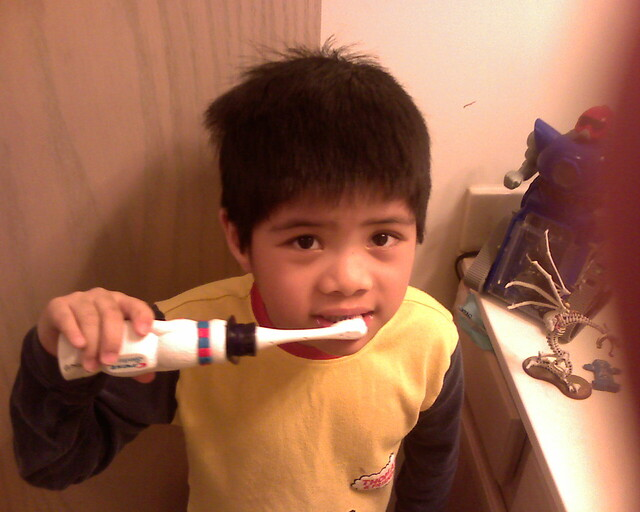
\includegraphics[scale=0.1]{images/toothbrush.jpg} }}%
    \qquad
    \subfloat{{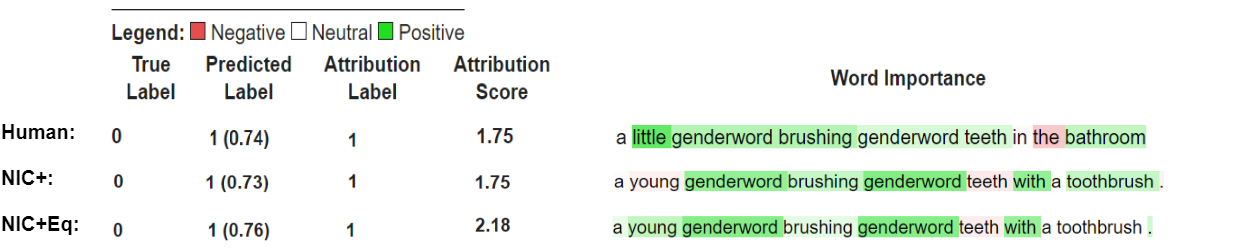
\includegraphics[scale=0.47]{images/QualitativeResults1.png} }}%
    \\
    \addtocounter{subfigure}{-1}
    \subfloat[\centering Image ID: 76632]{{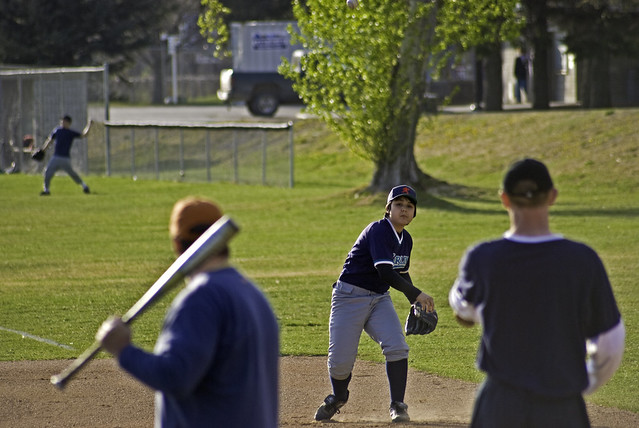
\includegraphics[scale=0.1]{images/baseball.jpg} }}%
    \qquad
    \subfloat{{\includegraphics[scale=0.47]{images/QualitativeResults2.png} }}%
    \caption{Integrated gradients example on two sets of image captions generated by a human, NIC+, and NIC+Equalizer respectively. The images that the captions describe can be seen on the left together with their corresponding image ID in the MSCOCO dataset.}%
    \label{fig:integrated:grads:qualitative}%
\end{figure}
%Let's decide on the order of the results later. Just fill it in for now.
\subsubsection{Quantifying the gender bias}
In order to better understand which of the two genders gets amplified and how much, we
ran our experiments on NIC, NIC+ and NIC+Equalizer, since they provide an overview of the best and 
the worst model and additionally NIC+ provides a baseline to NIC+Equalizer. In order to quantify 
bias we averaged the attribution scores for both genders as can be seen in Table \ref{table:attributionSums}. The average was obtained after running the model for 10 different 
seeds. These scores were obtained using the LSTM model. Unfortunately executing the algorithm on the 
BERT models was time consuming, hence, we are able to show the attribution scores for BERT-ft for only one seed, the results can be seen in Appendix C in Table \ref{table:attributionSumsBert}.

\begin{table}[H]
\begin{center}
\setlength{\tabcolsep}{4.25pt} % Default value: 6pt
\renewcommand{\arraystretch}{1.25} % Default value: 1
\begin{tabular}{lrrr}
\toprule
\multicolumn{1}{c}{} & 
\multicolumn{3}{c}{LSTM}
\\
\cmidrule(r){1-4} 
Model & Female & Male & Sum \\
\hline
NIC \cite{NIC:2015} & $1.12\pm0.0$ & $1.10\pm0.0$ & $2.22$ \\

NIC+ \cite{NICplusNICEqualizer:2018} & $1.20\pm0.0$ & $1.18\pm0.0$ & $2.38$\\

NIC+Equalizer \cite{NICplusNICEqualizer:2018} & $1.31\pm0.0$ & $1.22\pm0.0$ & $2.53$ \\

\bottomrule
\end{tabular}
\caption{Averages of attribution scores for the LSTM model. }
\label{table:attributionSums}
\end{center}
\end{table}

\subsubsection{Duplicates in the data set and the effect on LIC and attribution scores}
During our examination of the original code and methodology employed in the research, we encountered certain challenges. One of these challenges was the presence of duplicate entries in both the training and testing datasets. This limitation was brought to light through the gracious provision of access to the code and dataset by the original authors. \newline

To mitigate the issue, we implemented a solution that involved the elimination of all captions in the test set that overlapped with the captions in the training set. Subsequently, we re-calculated the $LIC_M$ scores to assess the impact of this modification. The results of this recalculation are shown in Table \ref{table:removeduplicates}.
%The results displayed in Table \ref{table:removeduplicates} were obtained by averaging over ten seeds. 

%and also display the number of non-training captions left of the 662 test samples. The third column shows the difference in $LIC_M$ score compared to the original results displayed in table \ref{table:lstmgender}. 

\begin{table}[H]
\begin{center}
\setlength{\tabcolsep}{6pt} % Default value: 6pt
\renewcommand{\arraystretch}{1.25} % Default value: 1
\begin{tabular}{lrrrrrrr}
\toprule
\multicolumn{1}{c}{} & 
\multicolumn{3}{c}{LSTM duplicate removal}


\\\cmidrule(r){2-4}
Model & $LIC_M$ & Unseen & Difference \\
\hline
NIC \cite{NIC:2015} & $40.0\pm1.9$ & $231\pm17$ & $-3.2$\\
SAT \cite{SAT:2015} & $41.4\pm2.3$ & $296\pm14$ & $-3.4$\\
FC \cite{Att2inFC:2016} & $38.8\pm2.5$ & $133\pm11$ & $-7$ \\
Att2in \cite{Att2inFC:2016} & $39.1\pm2.1$ & $214\pm13$ & $-6.6$ \\
UpDn \cite{UpDn:2017} & $42.9\pm1.7$ & $279\pm14$ & $-4.6$ \\
Transformer \cite{transformer:2017} & $43.5\pm0.8$ & $452\pm16$ & $-4.8$ \\
OSCAR \cite{OSCAR:2020} & $46.0\pm1.8$ & $373\pm15$ & \textcolor{numbergreen}{$-2.6$} \\
NIC+ \cite{NICplusNICEqualizer:2018} & $38.6\pm3.3$ & $133\pm10$ & $-7.7$ \\
NIC+Equalizer \cite{NICplusNICEqualizer:2018} & $39.2\pm2.6$ & $137\pm7$ & \textcolor{numberred}{$-12.7$} \\

\bottomrule
\end{tabular}
\caption{$LIC_M$ scores averaged over ten seeds after removing training samples from the test set. The average number of non-training samples are displayed in the "Unseen" column and the difference with our original $LIC_M$ is displayed with "Difference". The original test set size was 662 samples for each model.}´
\label{table:removeduplicates}
\end{center}
\end{table}

\section{Analysis}
The following section will elaborate more on the results mentioned earlier. First, the observed discrepancy in our reproduced results between NIC+Equalizer and Oscar with the pre-trained BERT as 
language encoder, is reasonable. In the original paper the observation is made that there is a trade-off between bias amplification and model performance.  Since OSCAR was the best performing model in terms of 
accuracy metrics, the higher LIC score is in line with this observation.
\newline

In Table \ref{table:attributionSums} we observe that the NIC+Equalizer model amplifies 
bias the most, which can also be noticed 
by looking at the sums of the attribution scores, where we observe that the scores are highest for NIC+Equalizer. These scores 
verify the claim of the authors that NIC+Equalizer amplifies bias beyond the baseline NIC+ from a different perspective, using 
integrated gradients. \newline

Finally, the results of the removal of duplicates, as presented in Table 
\ref{table:removeduplicates}, indicate a decline in the 
$LIC_M$ scores compared to the original results, despite similar training sets and models. The test sets decrease in size on 
average by 68\%, with the FC and NIC+ models having the most substantial reductions of around 80\%. This reduction in the test 
set size could potentially compromise the reliability of our results, as the decreased volume might result in increased variance 
and sensitivity to outliers. However, the decrease in the $LIC_M$ scores across all models suggests that the initial estimation 
of bias amplification may still have been overestimated.
\newline

\section{Discussion}

% Give your judgement on if your experimental results support the 
% claims of the paper. Discuss the strengths and weaknesses of your approach - perhaps you didn't have time to run all the experiments, or perhaps you did additional experiments that further strengthened the claims in the paper.
In this study, we aimed to replicate the findings presented in the work of Hirota et 
al. and extend it by incorporating the integrated gradients method developed by Merity 
et al. Our results indicate that the integrated gradients method provides valuable 
insight into the decision-making process of classification models and has the potential 
to mitigate the problem of bias amplification in captioning models in future studies. \newline

However, it is worth noting that the computational expense of this method, particularly when using BERT as the language encoder, is a limitation. The calculation of 
attribution scores and visualization took an excessive amount of time, which made it 
infeasible in this study to perform more attribution score analysis using BERT. \newline

Additionally, the presence of duplicate captions in the training and test sets raises concerns regarding the validity of the original results. Our brief experiment indicated a decline in the average $LIC_M$ scores by approximately 5 units, highlighting the potential for overfitting and overconfident predictions. Therefore, future research should address the issue of duplicate captions in the train and test splits and re-evaluate the reliability of these results to ensure the validity of the findings.


% The results of the integrated gradients visualization were unexpected. The "genderword" used as the mask for the LSTM classifier was found to be the word with the highest attribution score for predicting the female label in most test captions. To gain a better understanding of the impact of this word, "genderword" was replaced with an out-of-vocabulary token, specifically "[MASK]". Figure X illustrates that this change in a single word, as long as it is out-of-vocabulary, can result in a different prediction in 161 of the 662 human-generated captions analyzed. The first two captions in figure X depict the instance in which replacing "genderword" with "[MASK]" resulted in a correct prediction, while the last two captions demonstrate an example where the replacement led to an incorrect prediction. The overall results showed a decrease in the average bias score towards the female gender, from 50.6\% to 44.1\%, a decrease of 6.5\%. Conversely, the average confidence towards male subjects increased by 6.5\%.


\subsection{Communication with original authors}
Thanks to clear writing and accessible code/data, we were able to reproduce results without contacting the authors. We did however contact the authors to inform them of our work. Hirota's response promised to remove the data leakage in the human captions and as for the duplicates in the outputs of the captioning models, Hirota did not find it reasonable to remove those duplicates. The reason being that generating similar captions is something that captioning models tend to do in comparison to humans and this is one of the reasons for bias.
